\documentclass{beamer}
\usetheme{Madrid}
\usepackage{graphicx}
\usepackage{amsmath}
\usepackage{hyperref}
\usepackage{graphicx}
\usepackage{amsmath}
\usepackage{amsfonts}
\usepackage{tikz}
\usetikzlibrary{shapes, arrows, positioning, calc}


\title[NoMaD]{NoMaD: \textbf{N}avigati\textbf{o}n with Goal-\textbf{Ma}sked \textbf{D}iffusion}
\author{Sehaj Ganjoo, Shobhnik Kriplani, \\ Abhishek Kumar Jha, Namashivayaa V}
\institute{IISc Bengaluru \newline BTech. Mathematics and Computing}
\date{April 2025}

\begin{document}

\begin{frame}
\titlepage
\end{frame}

\begin{frame}{Motivation and Goal}
    \textbf{Robotic navigation in unfamiliar environments requires:}
    \begin{itemize}
        \item Task-oriented navigation — reaching specified goals
        \item Task-agnostic exploration — discovering and mapping new areas
    \end{itemize}
    \pause
    \begin{block}{The Challenge}
        These two objectives are typically handled by \textit{separate systems}.\\[1ex]
        Exploration can be decomposed into:
        \begin{itemize}
            \item \textbf{Local Exploration:} Learning short-horizon control policies for diverse actions
            \item \textbf{Global Planning:} Using those policies to achieve long-horizon, goal-directed behavior
        \end{itemize}
    \end{block}
    \pause
    \begin{block}{Key Question}
        Can a \textit{single model} unify both tasks — exploration and navigation?
    \end{block}
    \end{frame}
    \begin{frame}{What is NoMaD?}
        \textbf{NoMaD} is a transformer-based diffusion policy designed for long-horizon, memory-efficient navigation.\\[0.5em]
        It supports both:
        \begin{itemize}
            \item \textbf{Goal-conditioned navigation} — moving towards a specified visual goal
            \item \textbf{Open-ended exploration} — learning diverse behaviors without explicit goals
        \end{itemize}
        \pause
        \bigskip
        \texttt{NoMaD = \{EfficientNet + Vision Transformer\} $\leftarrow$ \textbf{ViNT} \\+ Diffusion Policies}
        \pause
        \bigskip
        \begin{block}{}
            It combines a transformer backbone to encode the high-dimensional visual stream, with diffusion models that predict a sequence of future actions in a generative manner.
        \end{block}
        \end{frame}

\begin{frame}{Overview of NoMaD Architecture}
    \begin{block}{Visual Goal-Conditioned Navigation}
        Backbone: ViNT (Visual Navigation Transformer)\\
        How does ViNT work?
        \begin{itemize}
            \item Recieves: A sequence of past and current observations $o_t$=$o_{t-P:t}$
            \item \textbf{Visual Encoder:} Each observation is processed using an EfficientNet-B0 encoder to extract feature embeddings.
        \end{itemize}
        \pause
        \texttt{EfficientNet?}
        \begin{itemize}
            \item A new method of Scaling CNNs to improve accuracy and efficiency
            \item It uses a \textbf{compound scaling} to uniformly scale all dimensions of depth, width, and resolution.
        \end{itemize}
    \end{block}
\end{frame}
\begin{frame}
    \begin{figure}
        \centering
        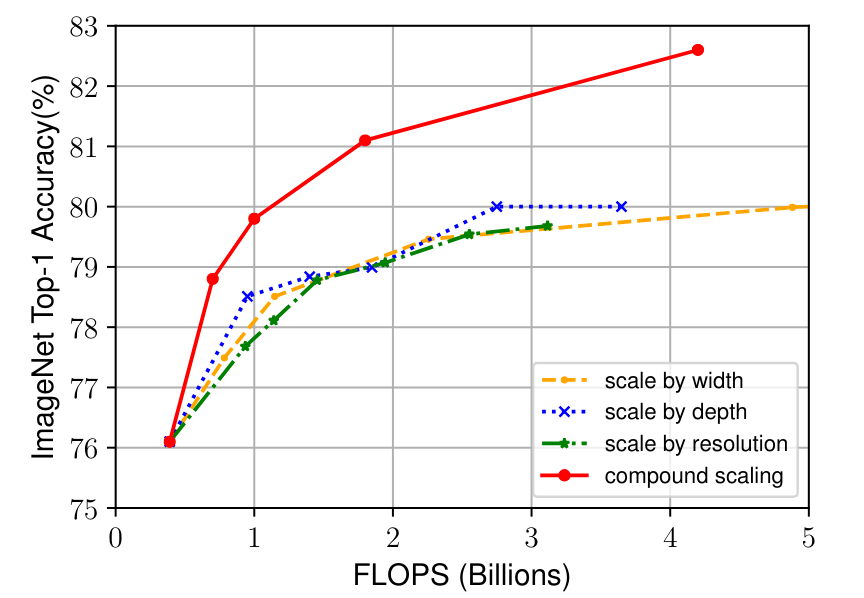
\includegraphics[width=0.8\linewidth]{effnet_scaling.png}
        \caption{Compound Scaling}
        \label{fig:efficientnet}
    \end{figure}
\end{frame}
\begin{frame}{EfficientNet}
    \begin{block}{}
        Use Network Architecture Search (NAS) to find the best baseline network (EfficientNet-B0)\\
        \bigskip
        \textbf{Optimization Objective:}
    \[
    \text{ACC}(m) \times \left[\frac{\text{FLOPS}(m)}{T}\right]^w
    \]
    \begin{itemize}
        \item $\text{ACC}(m)$: accuracy of model $m$
        \item $\text{FLOPS}(m)$: floating point operations
        \item $T$: target FLOPS
        \item $w = -0.07$: controls trade-off between accuracy and FLOPS
    \end{itemize}
    \end{block}
\end{frame}
\begin{frame}{EfficientNet Scaling}
    \begin{block}{\textbf{Compound Scaling}}
        EfficientNet introduces a principled way to scale up CNNs using a single compound coefficient $\phi$.
        \begin{itemize}
            \item Simultaneously scales:
            \begin{itemize}
                \item Network depth $d$
                \item Width $w$
                \item Input resolution $r$
            \end{itemize}
            \item Scaling formulas:
            \[
            d = \alpha^\phi, \quad w = \beta^\phi, \quad r = \gamma^\phi
            \]
            \item Constants $\alpha$, $\beta$, and $\gamma$ are determined via grid search.
        \end{itemize}
        \vspace{0.3em}
        \textbf{Subject to constraint:}
        \[
        \alpha \cdot \beta^2 \cdot \gamma^2 \approx 2
        \]
        Ensures that the model scales within a fixed computational budget.
    \end{block}
\end{frame}
\begin{frame}
    \begin{figure}
        \centering
        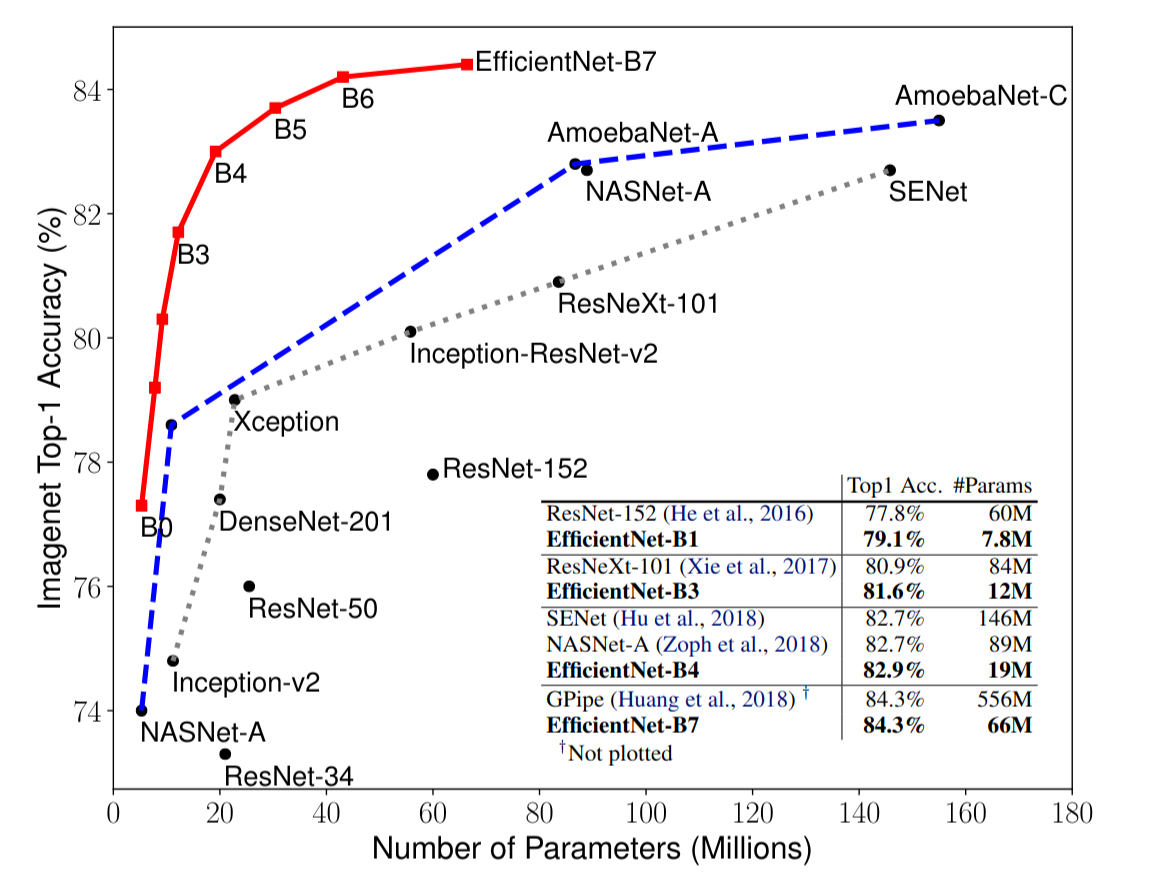
\includegraphics[width=0.8\linewidth]{effnet_imagenet.png}
        \caption{Accuracy on imagenet}
        \label{fig:efficientnet}
    \end{figure}
\end{frame}


\begin{frame}{Overview of NoMaD Architecture}
    \begin{block}{Visual Goal-Conditioned Navigation}
        Backbone: ViNT (Visual Navigation Transformer)\\
        How does ViNT work?
        \begin{itemize}
            \item Recieves: A sequence of past and current observations $o_t$=$o_{t-P:t}$
            \item \textbf{Visual Encoder:} Each observation is processed using an EfficientNet-B0 encoder to extract feature embeddings.
            \pause
            \item \textbf{Goal Fusion:} The current and goal images are combined using a goal-fusion encoder.
            \item \textbf{Transformer Attention:} These fused features (tokens) are passed through a Transformer model to generate a context vector $c_t$.
            \item \textbf{Predictions:} The context vector is used to predict:\\
            -A distribution over future actions: $a_t = f_a(c_t)$\\
            -An estimate of temporal distance to the goal: $d(o_t, o_g) = f_d(c_t)$
        \end{itemize}
    \end{block}
\end{frame}
\begin{frame}{Extending to Long-Horizon Planning with Topological Memory}
    \alert{However, ViNT is inherently goal-conditioned—it cannot operate in the absence
    of a goal image, limiting its ability to explore autonomously.}
    \pause
    \begin{block}{Solution}
        To enable open-ended exploration, NoMaD incorporates a Topological Memory $\mathcal{M}$:
        \begin{enumerate}
            \item Nodes represent previously encountered visual observations.
            \item Edges represent traversable paths, established using ViNT's predicted distances.
        \end{enumerate}
        This enables:
        \begin{itemize}
            \item \textbf{Subgoal Planning:} The model can plan a sequence of subgoals to reach a target location.
            \item \textbf{Frontier Exploration:} The model can autonomously explore new areas by identifying frontiers in the topological map.
        \end{itemize}
    \end{block}
\end{frame}
\begin{frame}{Overview of NoMaD Architecture}
    \texttt{NoMaD = \{\textcolor{green}{EfficientNet + Vision Transformer}\} $\leftarrow$ \textbf{ViNT} \\+ Diffusion Policies}\\
    Nomad builds upon ViNT by:\\
    \textbf{Attention based Goal Masking:}\\
    Introduces a binary mask $m$, and modifies the context vector $c_t$ as:
    \[c_t = f(\psi(o_i),\phi(o_t,o_g),m)\]
    \begin{figure}
        \centering
        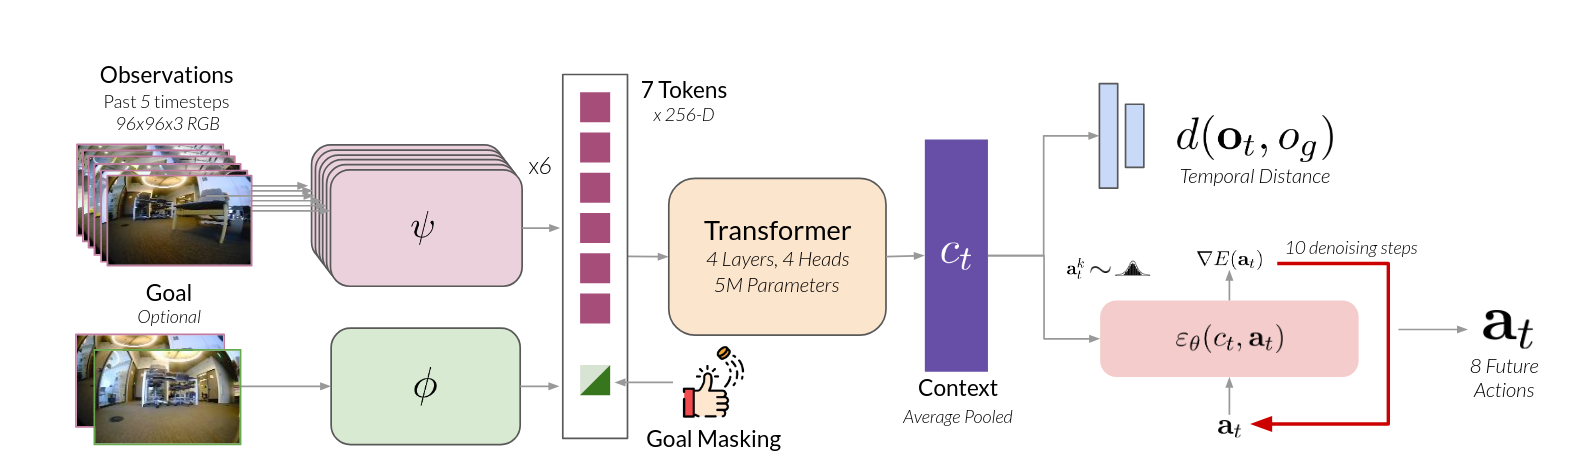
\includegraphics[width=1.01\linewidth]{nomad_diagram.png}
    \end{figure}
\end{frame}

\begin{frame}{Overview of NoMaD Architecture}
    \texttt{NoMaD = \{EfficientNet + Vision Transformer\} $\leftarrow$ \textbf{ViNT} \\+ \textcolor{green}{Diffusion Policies}}\\
    \textbf{Diffusion Policies:}\\
    To model complex, multimodal action distributions, NoMaD employs a diffusion model to approximate the conditional distri-
    bution of the next action as: $p(a_t|c_t)$.\\
    \textbf{1. Forward Process}: Start with a real action $a^{0}_t$ and add gaussian noise to it over multiple steps.
        \begin{center}
            $a^{k}_t = \sqrt{\alpha_k} a^{k-1}_t + (\sqrt{1 - \alpha_k}) \epsilon$
        \end{center}
        where:\\
    \begin{itemize}
        \item $\epsilon$ $\sim$ $\mathcal{N}$(0,I) is a random noise
        \item $\alpha_k$ is a noise scheduler (eg square cosine)
        \item By step K, the action is almost pure noise.
    \end{itemize}
\end{frame}
\begin{frame}{Overview of NoMaD Architecture}
    \texttt{NoMaD = \{EfficientNet + Vision Transformer\} $\leftarrow$ \textbf{ViNT} \\+ \textcolor{green}{Diffusion Policies}}\\
    \textbf{2. Reverse Denoising:} starting from pure noise $a^{k}_t$ $\sim$ $\mathcal{N}(0,I)$, it denoises step by step to recover the final clean action $a^{0}_t$.\\
    Each denoising step is :
    \begin{center}
        \[a^{k-1}_t = \alpha(\alpha^{k}_t-\gamma_k.\epsilon_{\theta}(c_t, a^{k}_t,k)) + \mathcal{N}(0,\sigma^2.I)\]
    \end{center}
    Where:
    \begin{itemize}
        \item Here, $\epsilon_\theta$ is the noise prediction network conditioned on the context $c_t$, which may or may not include the goal depending on $m$.
        \begin{itemize}
            \item It is a 1D conditional U-Net with 15 CNN layers.
            \item Input:Noisy action $a^{k}_t$, Context vector $c_t$, and the diffusion step k.
            \item the predicted noise vector $\hat{\epsilon}_k$,During training, it is compared to the true noise added earlier.
        \end{itemize}
        \item $\gamma, \alpha ,\sigma$ are scheduler constants.
    \end{itemize}
     
\end{frame}

\begin{frame}{Overview of NoMaD Architecture}
    \texttt{NoMaD = \{EfficientNet + Vision Transformer\} $\leftarrow$ \textbf{ViNT} \\+ \textcolor{green}{Diffusion Policies}}\\
    \textbf{3. Action Decoder:} The denoised action $a^{0}_t$ is then passed through a low-level action decoder to generate the final action $a_t$.
    \begin{itemize}
        \item The decoder maps the denoised action to a low-level control command for the robot.
        \item It can be a simple feedforward network or a more complex recurrent network.
    \end{itemize}
    \begin{figure}
        \centering
        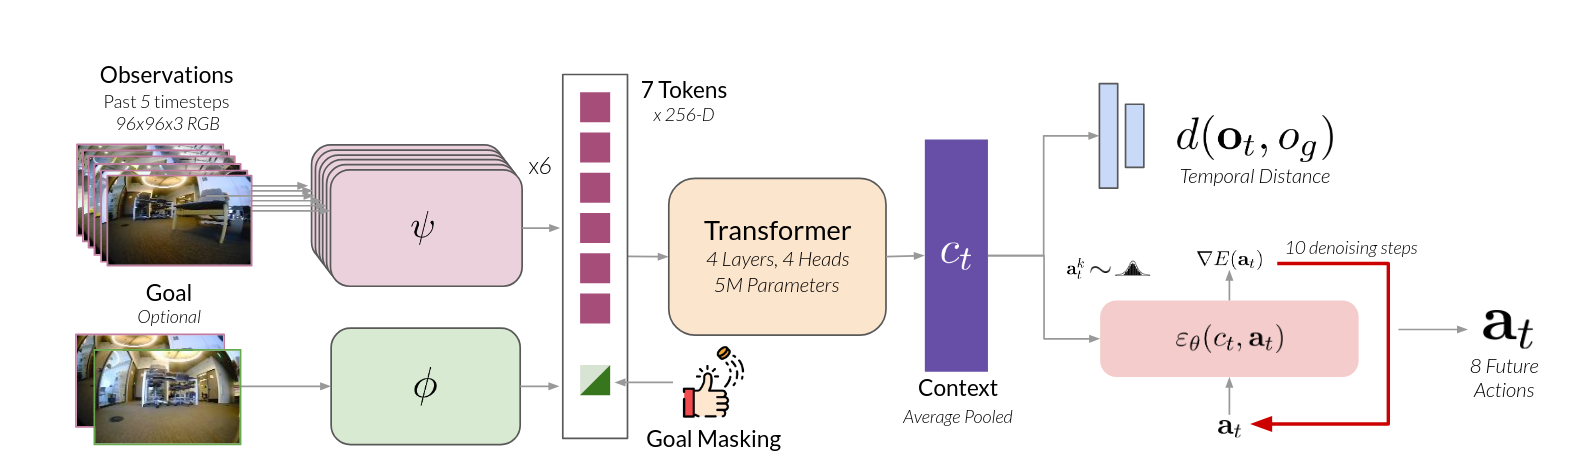
\includegraphics[width=1.01\linewidth]{nomad_diagram.png}
    \end{figure}
\end{frame}

\begin{frame}{Training Details and Experiments}
\begin{itemize}
    \item Datasets used: Sacson/HuRoN, RECON and SCAND
    \item Batch size: 47, Epochs: 10
    \item Optimizer: AdamW, Lr: $10^{-4}$ 
    \item Scheduler: Cosine annealing
\end{itemize}
\begin{figure}
    \centering
    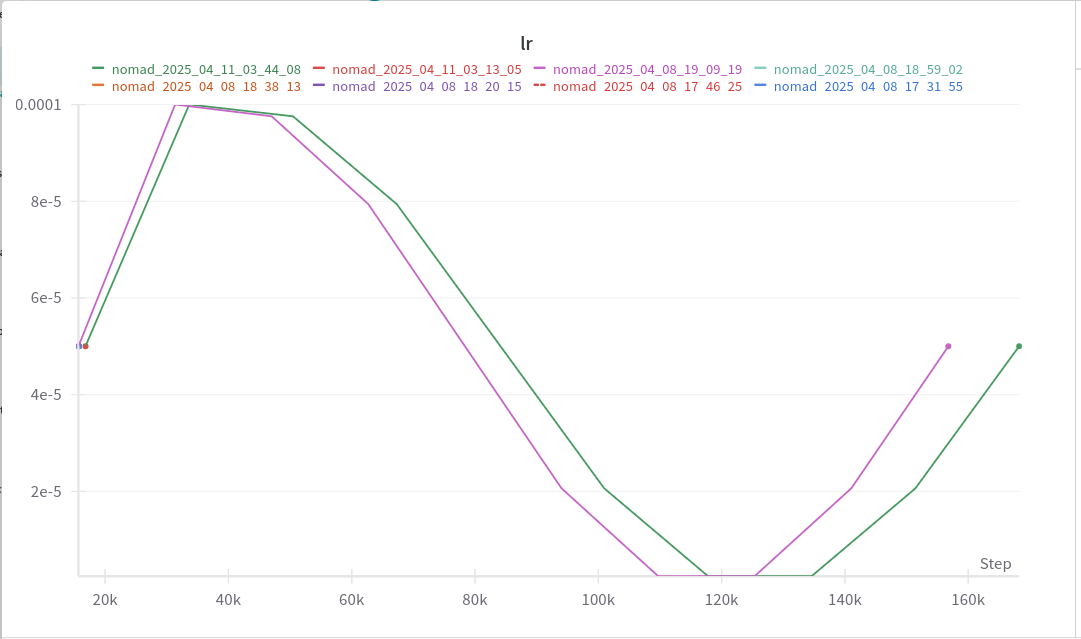
\includegraphics[width=0.8\linewidth]{lrdecay.png}
    \caption{Lr decay using cosine annealing}
    \label{fig:lrdecay}
\end{figure}
\end{frame}
\begin{frame}{Training Details and Experiments}
    \begin{itemize}
        \item Goal Masking Probability: $p_m$ = 0.5
        \item Diffusion Steps: 10
        \item Noise Scheduler: Square Cosine
    \end{itemize}
    \pause
    \begin{block}{Training Objective}
        \begin{itemize}
            \item \textbf{Diffusion Loss:} Measures the difference between the predicted and true noise.
            \item \textbf{Distance Loss:} Measures the difference between the predicted and true distance to the goal.
        \end{itemize}
    \end{block}
    \[ \mathcal{L}_{NoMaD}(\phi,\psi,f,\theta,f_d) = MSE(\epsilon^{k}, \epsilon_{\theta}(c_t, a^{0}_t + \epsilon^{k},k)) + \lambda .MSE(d(o_t, o_g), f_{d}(c_t))\]
    where:\\
    \begin{itemize}
        \item We set $\lambda$ to $10^{-4}$
        \item $\psi$,\ $\phi$ correspond to the visual encoders for the observation and goal images.
        \item $f$ corresponds to the transformer layers, $\theta$ to diffusion parameters,
        \item $f_d$ corresponds to the temporal distance predictor.
    \end{itemize}
\end{frame}

\begin{frame}{Experiments and Results}
\textbf{Metrics:}
\begin{itemize}
    \item Diffusion Loss $\approx 1.11$
    \item Distance Loss $\approx 128$
    \item Cosine Similarity $\approx 0.47$
\end{itemize}
\end{frame}


\begin{frame}{Comparision with ViNT}
    \textbf{Comparison with ViNT:}
\begin{itemize}
    \item Similar performance in goal-conditioned tasks
    \item No performance degradation when adding diffusion
\end{itemize}
\end{frame}
\begin{frame}{Challenges Faced}
\begin{itemize}
    \item CUDA Out Of Memory errors on limited GPU
    \item Module import issues with nested folder structures
    \item Gradients not propagating due to detached variables
\end{itemize}
\end{frame}

\begin{frame}{Team Contributions}
    \textbf{Shobhnik Kriplani:} \\
    \begin{itemize}
        \item Implemented the NoMaD architecture
        \item Developed the training pipeline
        \item Conducted experiments and analysis
    \end{itemize}
    
    \textbf{Sehaj Ganjoo:} \\
    \begin{itemize}
        \item Implemented the ViNT architecture
        \item Developed the goal fusion encoder
        \item Conducted experiments and analysis
    \end{itemize}
    
\end{frame}

\begin{frame}{Conclusion and Future Work}
\begin{itemize}
    \item Successfully trained NOMAD using diffusion for visual navigation
    \item Showed compatibility with ViNT-based perception
    \item Future work:
    \begin{itemize}
        \item Evaluate in simulation / real-world
        \item Improve runtime performance
        \item Try larger ViTs and alternate decoders
    \end{itemize}
\end{itemize}
\end{frame}

\begin{frame}{Q\&A}
Thank you! \newline
\textit{Questions are welcome.}
\end{frame}

\end{document}